
% this file is called up by thesis.tex
% content in this file will be fed into the main document
%----------------------- introduction file header -----------------------
%%%%%%%%%%%%%%%%%%%%%%%%%%%%%%%%%%%%%%%%%%%%%%%%%%%%%%%%%%%%%%%%%%%%%%%%%
%  Capítulo 1: Introducción- DEFINIR OBJETIVOS DE LA TESIS              %
%%%%%%%%%%%%%%%%%%%%%%%%%%%%%%%%%%%%%%%%%%%%%%%%%%%%%%%%%%%%%%%%%%%%%%%%%

\chapter{Introducción}

%: ----------------------- HELP: latex document organisation
% the commands below help you to subdivide and organise your thesis
%    \chapter{}       = level 1, top level
%    \section{}       = level 2
%    \subsection{}    = level 3
%    \subsubsection{} = level 4
%%%%%%%%%%%%%%%%%%%%%%%%%%%%%%%%%%%%%%%%%%%%%%%%%%%%%%%%%%%%%%%%%%%%%%%%%
%                           Presentación                                %
%%%%%%%%%%%%%%%%%%%%%%%%%%%%%%%%%%%%%%%%%%%%%%%%%%%%%%%%%%%%%%%%%%%%%%%%%

\section{Presentación} % section headings are printed smaller than chapter names

El progreso de la tecnología en las últimas décadas ha hecho posible que las máquinas realizen tareas que anteriormente eran confiadas solo a los seres humanos. La primera concepción de la palabra robot proviene de la obra \textsl{Rossum’s Universal Robots} del novelista checo Karel Capek[1]. En la lengua checha \textsl{robota} significa trabajo, y la RAE [2] define a un robot como \textsl{Máquina o ingenio electrónico programable, capaz de manipular objetos y realizar operaciones antes reservadas solo a las personas.}
\\

En la industria, los robots más utilizados son conocidos como robots manipuladores,
cuya estructura se asemeja a los brazos humanos como se muestra en la figura (\ref{robot1}) [3]. Su estructura está formada por eslabones unidos mediante articulaciones para brindar
libertad de movimiento en el entorno de trabajo, donde uno de los extremos del manipulador permanece fijo mientras que el otro extremo cuenta con una herramienta que le permite realizar una tarea para la que fue programado. Los robots manipuladores son utilizados en gran parte de las tareas como seleccionar y distribuir objetos, o para realizar modificaciones en su entorno como pintar o ensamblar, entre muchas otras, reduciendo los tiempos de operación y minimizando la necesidad de supervisión.
\\

Un robot manipulador se constituye de tres sistemas fundamentales. El primero es un sistema mecánico que le da forma al cuerpo del robot y está constituido pricipalmente por eslabones y articulaciones que permiten el movimiento en su espacio de trabajo, aunque también forman parte del sistema mecánico elementos de transmisión de potencia, como engranes, cadenas y poleas; elementos que otorgan estabilidad al robot, como los sistemas de contrapesos, ya sean fijos o móviles; y elementos de unión, como soldadura y tornillos. El segundo es un sistema eléctrico-electrónico que otorga energía para el movimiento de los motores, para la activación de sensores y la distribución de señales. El tercer sistema pertenece al control, que describe de manera matemática al robot y permite su manipulación para la realización de una tarea asignada.

\begin{figure}
	\centering
	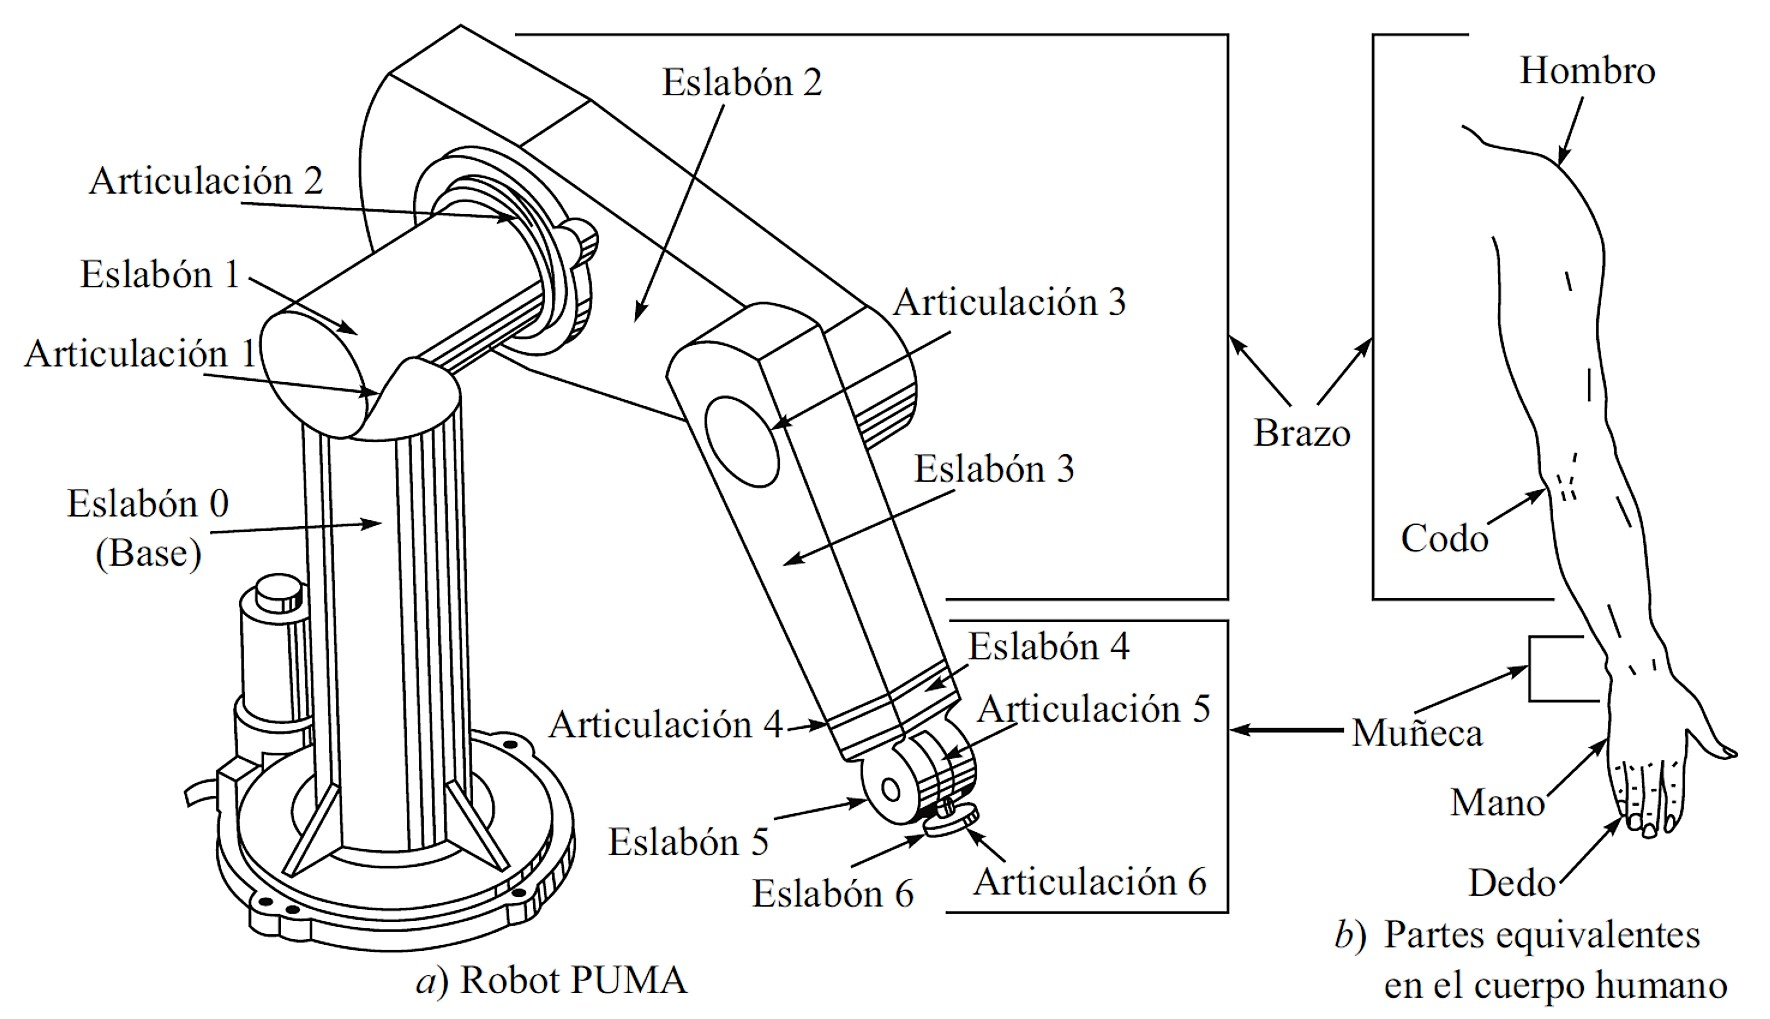
\includegraphics[scale=0.3]{Capitulo1/figs/Robot.jpg}      %Ruta completa de la imagen, porque se compila desde el archivo tesis.tex
	\caption{Manipulador robótico y sus partes equivalentes en el cuerpo humano}            %Pie de imagen
	\label{robot1}                            %nombre de referencia
\end{figure}

A pesar de la existencia de robots comerciales de tipo industrial, diseñar controladores para robots sigue siendo un área compleja y constantemente estudiada por parte de los constructores de robots, así como por centros de investigación en control y robótica alrededor del mundo. Podría argumentarse que los robots industriales actuales son capaces de realizar correctamente una gran variedad de tareas, por lo que pareciera innecesario el desarrollo de investigaciones sobre el tema de control de robots. Sin embargo, este último tema, además de interesante, tiene muchos retos que ofrecer en el marco teórico, y más importante aún, su estudio es indispensable en aplicaciones específicas que no pueden ser llevadas a cabo mediante los robots comerciales actuales.

%%%%%%%%%%%%%%%%%%%%%%%%%%%%%%%%%%%%%%%%%%%%%%%%%%%%%%%%%%%%%%%%%%%%%%%%%
%                           Objetivo                                    %
%%%%%%%%%%%%%%%%%%%%%%%%%%%%%%%%%%%%%%%%%%%%%%%%%%%%%%%%%%%%%%%%%%%%%%%%%

\section{Objetivo}

Diseño, manufactura y control de un robot manipulador con 5 grados de libertad capaz de realizar seguimiento de trayectorias.
%%%%%%%%%%%%%%%%%%%%%%%%%%%%%%%%%%%%%%%%%%%%%%%%%%%%%%%%%%%%%%%%%%%%%%%%%
%                           Motivación y estado del arte                %
%%%%%%%%%%%%%%%%%%%%%%%%%%%%%%%%%%%%%%%%%%%%%%%%%%%%%%%%%%%%%%%%%%%%%%%%%
\newpage

\section{Motivación}

Los robots manipuladores tienen un amplio uso en la industria y en áreas donde se pretende replicar el trabajo que realiza una persona, ya sea porque es demasiado complejo o se trata de procesos donde se requiera una gran precisión, por encontrarse en ambientes peligrosos o tóxicos, etcétera. Sin embargo, los robots manipuladores también pueden ser de gran utilidad en el ámbito educativo. Los estudiantes de robótica suelen tener acceso nulo o restringido a manipuladores ya sea por su delicadeza o por la intención de no dañaar al robot debido a los elevados costos de reparación. La creación de un manipulador con 5 grados de libertad a un bajo costo pondrá al alcance de los estudiantes una herramienta práctica en el área de la robótica industrial.
 
%%%%%%%%%%%%%%%%%%%%%%%%%%%%%%%%%%%%%%%%%%%%%%%%%%%%%%%%%%%%%%%%%%%%%%%%%
%                   Planteamiento del problema                          %
%%%%%%%%%%%%%%%%%%%%%%%%%%%%%%%%%%%%%%%%%%%%%%%%%%%%%%%%%%%%%%%%%%%%%%%%%

\section{Planteamiento del problema}

El diseño de robots manipuladores es una temática ampliamente abarcada en los trabajos escolares de nivel licenciatura, aunque la mayor parte de esa literatura tiene por objetivo demostrar conceptualmente las capacidades de los robots manipuladores. La construcción del prototipo funcional es un elemento que no se suele llevar a término.

%%%%%%%%%%%%%%%%%%%%%%%%%%%%%%%%%%%%%%%%%%%%%%%%%%%%%%%%%%%%%%%%%%%%%%%%%
%                           Metodología                                 %
%%%%%%%%%%%%%%%%%%%%%%%%%%%%%%%%%%%%%%%%%%%%%%%%%%%%%%%%%%%%%%%%%%%%%%%%%
\section{Metodología}

El proceso de construcción del manipulador comienza con el diseño, para ello se plantean los requerimientos y se traducen a especificaciones del robot. Posteriormente se elabora un diseño asistido por computadora donde se obtiene la geometría y espacio de trabajo del manipulador. Se realiza la descripción analítica del movimiento mediante la cinemática directa e inversa, se manufacturan las piezas y se ensambla el prototipo. Finalmente, se realiza la instrumentación, se diseña el control y se pone en marcha. %otra forma de poenr acentos

%%%%%%%%%%%%%%%%%%%%%%%%%%%%%%%%%%%%%%%%%%%%%%%%%%%%%%%%%%%%%%%%%%%%%%%%%
%                         Contribuciones                                %
%%%%%%%%%%%%%%%%%%%%%%%%%%%%%%%%%%%%%%%%%%%%%%%%%%%%%%%%%%%%%%%%%%%%%%%%%

\section{Contribuciones}

La principal contribución de este trabajo es la simplificación del proceso de construcción para un robot manipulador con 5 grados de libertad, con los elementos necesarios para ser replicado en posteriores trabajos y reduciendo los costos asociados a la fabricación, ademas de ser de código abierto para posteriores modificaciónes.

%%%%%%%%%%%%%%%%%%%%%%%%%%%%%%%%%%%%%%%%%%%%%%%%%%%%%%%%%%%%%%%%%%%%%%%%%
%                           Estructura de la tesis                      %
%%%%%%%%%%%%%%%%%%%%%%%%%%%%%%%%%%%%%%%%%%%%%%%%%%%%%%%%%%%%%%%%%%%%%%%%%

\section{Estructura de la tesis}

En este capítulo se hace una breve descripción del trabajo a desarrollar, el objetivo y algunas ideas generales de robots manipuladores, en el siguiente capítulo se encuentran los fundamentos teóricos que sirven para entender las generalidades de los manipuladores, su composición y la forma de operarlos. En el tercer capítulo se aborda el diseño mecánico junto con un análisis de los elementos que conforman al manipulador, las geometrías y los espacios de trabajo que definirán la movilidad. En el capítulo cuatro se lleva a cabo la construcción del prototipo. En el quinto capitulo se habla del control, la instrumentación y la programación del manipulador. En el sexto capítulo se analizan los resultados obtenidos donde se observa la capacidad real del robot manipulador construido y en el último capítulo se tratan las conclusiones y el posible trabajo a futuro del proyecto.